\section{Casos de uso}

\begin{figure}[H]
  \centering
  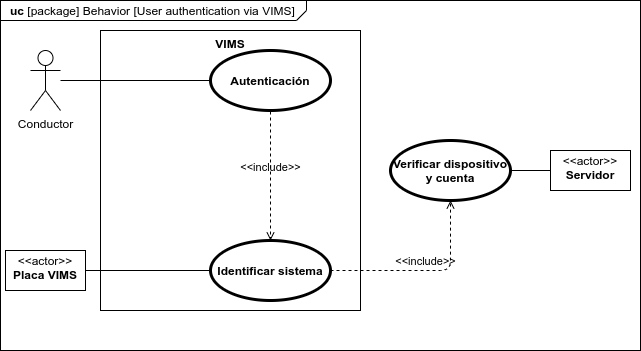
\includegraphics[width=\linewidth]{diagrams/UseCases-UC1 - auth.png}
  \caption{Caso de uso \texttt{01} -- \textit{autenticación}.}
  \label{uc:auth}
\end{figure}

\begin{table}[H]
  \centering
  \begin{tabularx}{\textwidth}{|c|c|X|}
    \hline
    \texttt{01}                                & \multicolumn{2}{c|}{\textit{Autenticación}}                                                                                                                                                                                                                 \\
    \hline
    \textbf{Descripción}                       & \multicolumn{2}{X|}{La placa identificará de forma inequívoca al conductor (usuario) y a sí misma frente al servidor.}                                                                                                                                      \\
    \hline
    \multirow{5}{*}{\textbf{Secuencia normal}} & \textbf{Paso}                                                                                                          & \textbf{Acción}                                                                                                                    \\
    \cline{2-3}
                                               & 1                                                                                                                      & \multicolumn{1}{L|}{El usuario se autentica contra la placa con su cuenta personal ya creada.}                                     \\
    \cline{2-3}
                                               & 2                                                                                                                      & \multicolumn{1}{L|}{La placa \ac{VIMS} recoge la información del usuario y la envía al servidor junto con su identificador único.} \\
    \cline{2-3}
                                               & 3                                                                                                                      & \multicolumn{1}{L|}{El servidor verifica que la cuenta del usuario existe y se asocia la información al dispositivo.}              \\
    \cline{2-3}
                                               & 4                                                                                                                      & \multicolumn{1}{L|}{La placa almacena la información del usuario y finaliza el proceso de inicio de sesión.}                       \\
    \hline
    \multirow{2}{*}{\textbf{Excepciones}}      & \textbf{Paso}                                                                                                          & \textbf{Acción}                                                                                                                    \\
    \cline{2-3}
                                               & 2 & \multicolumn{1}{L|}{La placa no cuenta con conexión a la red o el servidor no está disponible.} \\
    \cline{2-3}
                                               & 3                                                                                                                      & \multicolumn{1}{L|}{La cuenta del usuario no existe.}                                                                                                                                   \\
    \hline
  \end{tabularx}
\end{table}